%% LyX 2.3.6.1 created this file.  For more info, see http://www.lyx.org/.
%% Do not edit unless you really know what you are doing.
\documentclass[english]{article}
\usepackage[T1]{fontenc}
\usepackage[latin9]{inputenc}
\usepackage{float}
\usepackage{amssymb}
\usepackage{graphicx}

\makeatletter
\@ifundefined{showcaptionsetup}{}{%
 \PassOptionsToPackage{caption=false}{subfig}}
\usepackage{subfig}
\makeatother

\usepackage{babel}
\begin{document}
\title{Advanced Deep Learning\\
Homework 2}
\author{Abbas Nosrat\\
810199294}

\maketitle
\pagebreak{}

\tableofcontents{}

\pagebreak{}

\section{Generative Adversarial Networks}

\subsection{Stage 1}
\begin{itemize}
\item The loss function used in cyclegan is consisted of three parts:
\begin{itemize}
\item \textbf{Adversarial Loss}: This loss is formulated as
\[
\mathcal{L_{GAN}}=\mathbb{E}_{y\sim P_{data}(y)}\left[\left(D(y)-1\right)^{2}\right]+\mathbb{E}_{X\sim P_{data}(X)}\left[\left(D(G(X))\right)^{2}\right]
\]
This loss is applied to the output of the discriminator and it is
basically a classification loss which gives a hard 1 label to the
real images and a hard zero label to the generated images which tries
to train the discriminator to distinguish between fake and real images.
Optimizing this loss for the generator, trains the generator to generate
images that will increase the discriminator loss .This loss is responsible
for the adversarial nature of cyclegan and without this loss, the
generators and discriminators cannot be trained. There are two $\mathcal{L_{GAN}}$
terms corresponding to the two pairs of generator and discriminators.
\item \textbf{Cycle Consistency Loss:} This loss is and L1 loss between
the input image and the output of the second generator. It tries to
learn the networks to return the image to its original state after
passing it through both generators. In other words 
\[
G_{2}(G_{1}(X))\approx X\Rightarrow\mathcal{L}_{cycle}=\left\Vert X-G_{2}(G_{1}(X))\right\Vert 
\]
The general idea of GANs is that the network can learn any mapping
from the input domain to the target domain. However, the network may
learn to change the spatial properties of the image such that the
output image looks nothing like the input image. In order to prevent
such phenomena, cycle consistency loss is utilized. Utilization of
this loss, enforces the network to only apply the minimum change required
to go from the input domain to the target domain. By removing this
term from the objective function, the network may learn to change
the image too much.
\item \textbf{Identity Loss:} This loss ensures that if an image from the
target domain is given as input to the generator, the image remains
unchanged. This loss has no positive effect on training of the networks
and in some cases it is better to be removed.
\end{itemize}
\item The authors of cycleGAN used MSE loss instead of cross entropy due
to training stability. Optimizing MSE loss is more stable than BCE
and would result in generation of better quality images.
\item If an objective is consisted of multiple terms, it is generally represented
as a weighted sum. By increasing the weight for the the more important
terms and/or decreasing for the less important ones, one can ensure
better training and fulfillment of the desired objective.
\item Yes. The generator uses a hierarchical architecture. It reduces dimensions
at first and then increases them to match the target image. Any CNN
architecture following the same pattern can be used. A good example
of this type of networks can be UNET. For the discriminator part,
any classifier architecture can be used since it is a classification
problem. However, the results may be worse than PatchGan. Another
approach can be the use of Siamese networks. The objective can be
reformulated. In the new formulation, Instead of classification loss
for the discriminator, Triplet loss or Contrastive loss can be used.
By changing the loss in this way, the discriminator tries to create
distance between real and fake images and the generator tries to get
its images among the real images.
\end{itemize}

\subsection{Stage 2}
\begin{itemize}
\item The model has been trained for 20 epochs due to lack of computational
power and time. The identity loss was removed to reduce computations
and save time. The results are demonstrated in figure 1:
\begin{figure}[h]
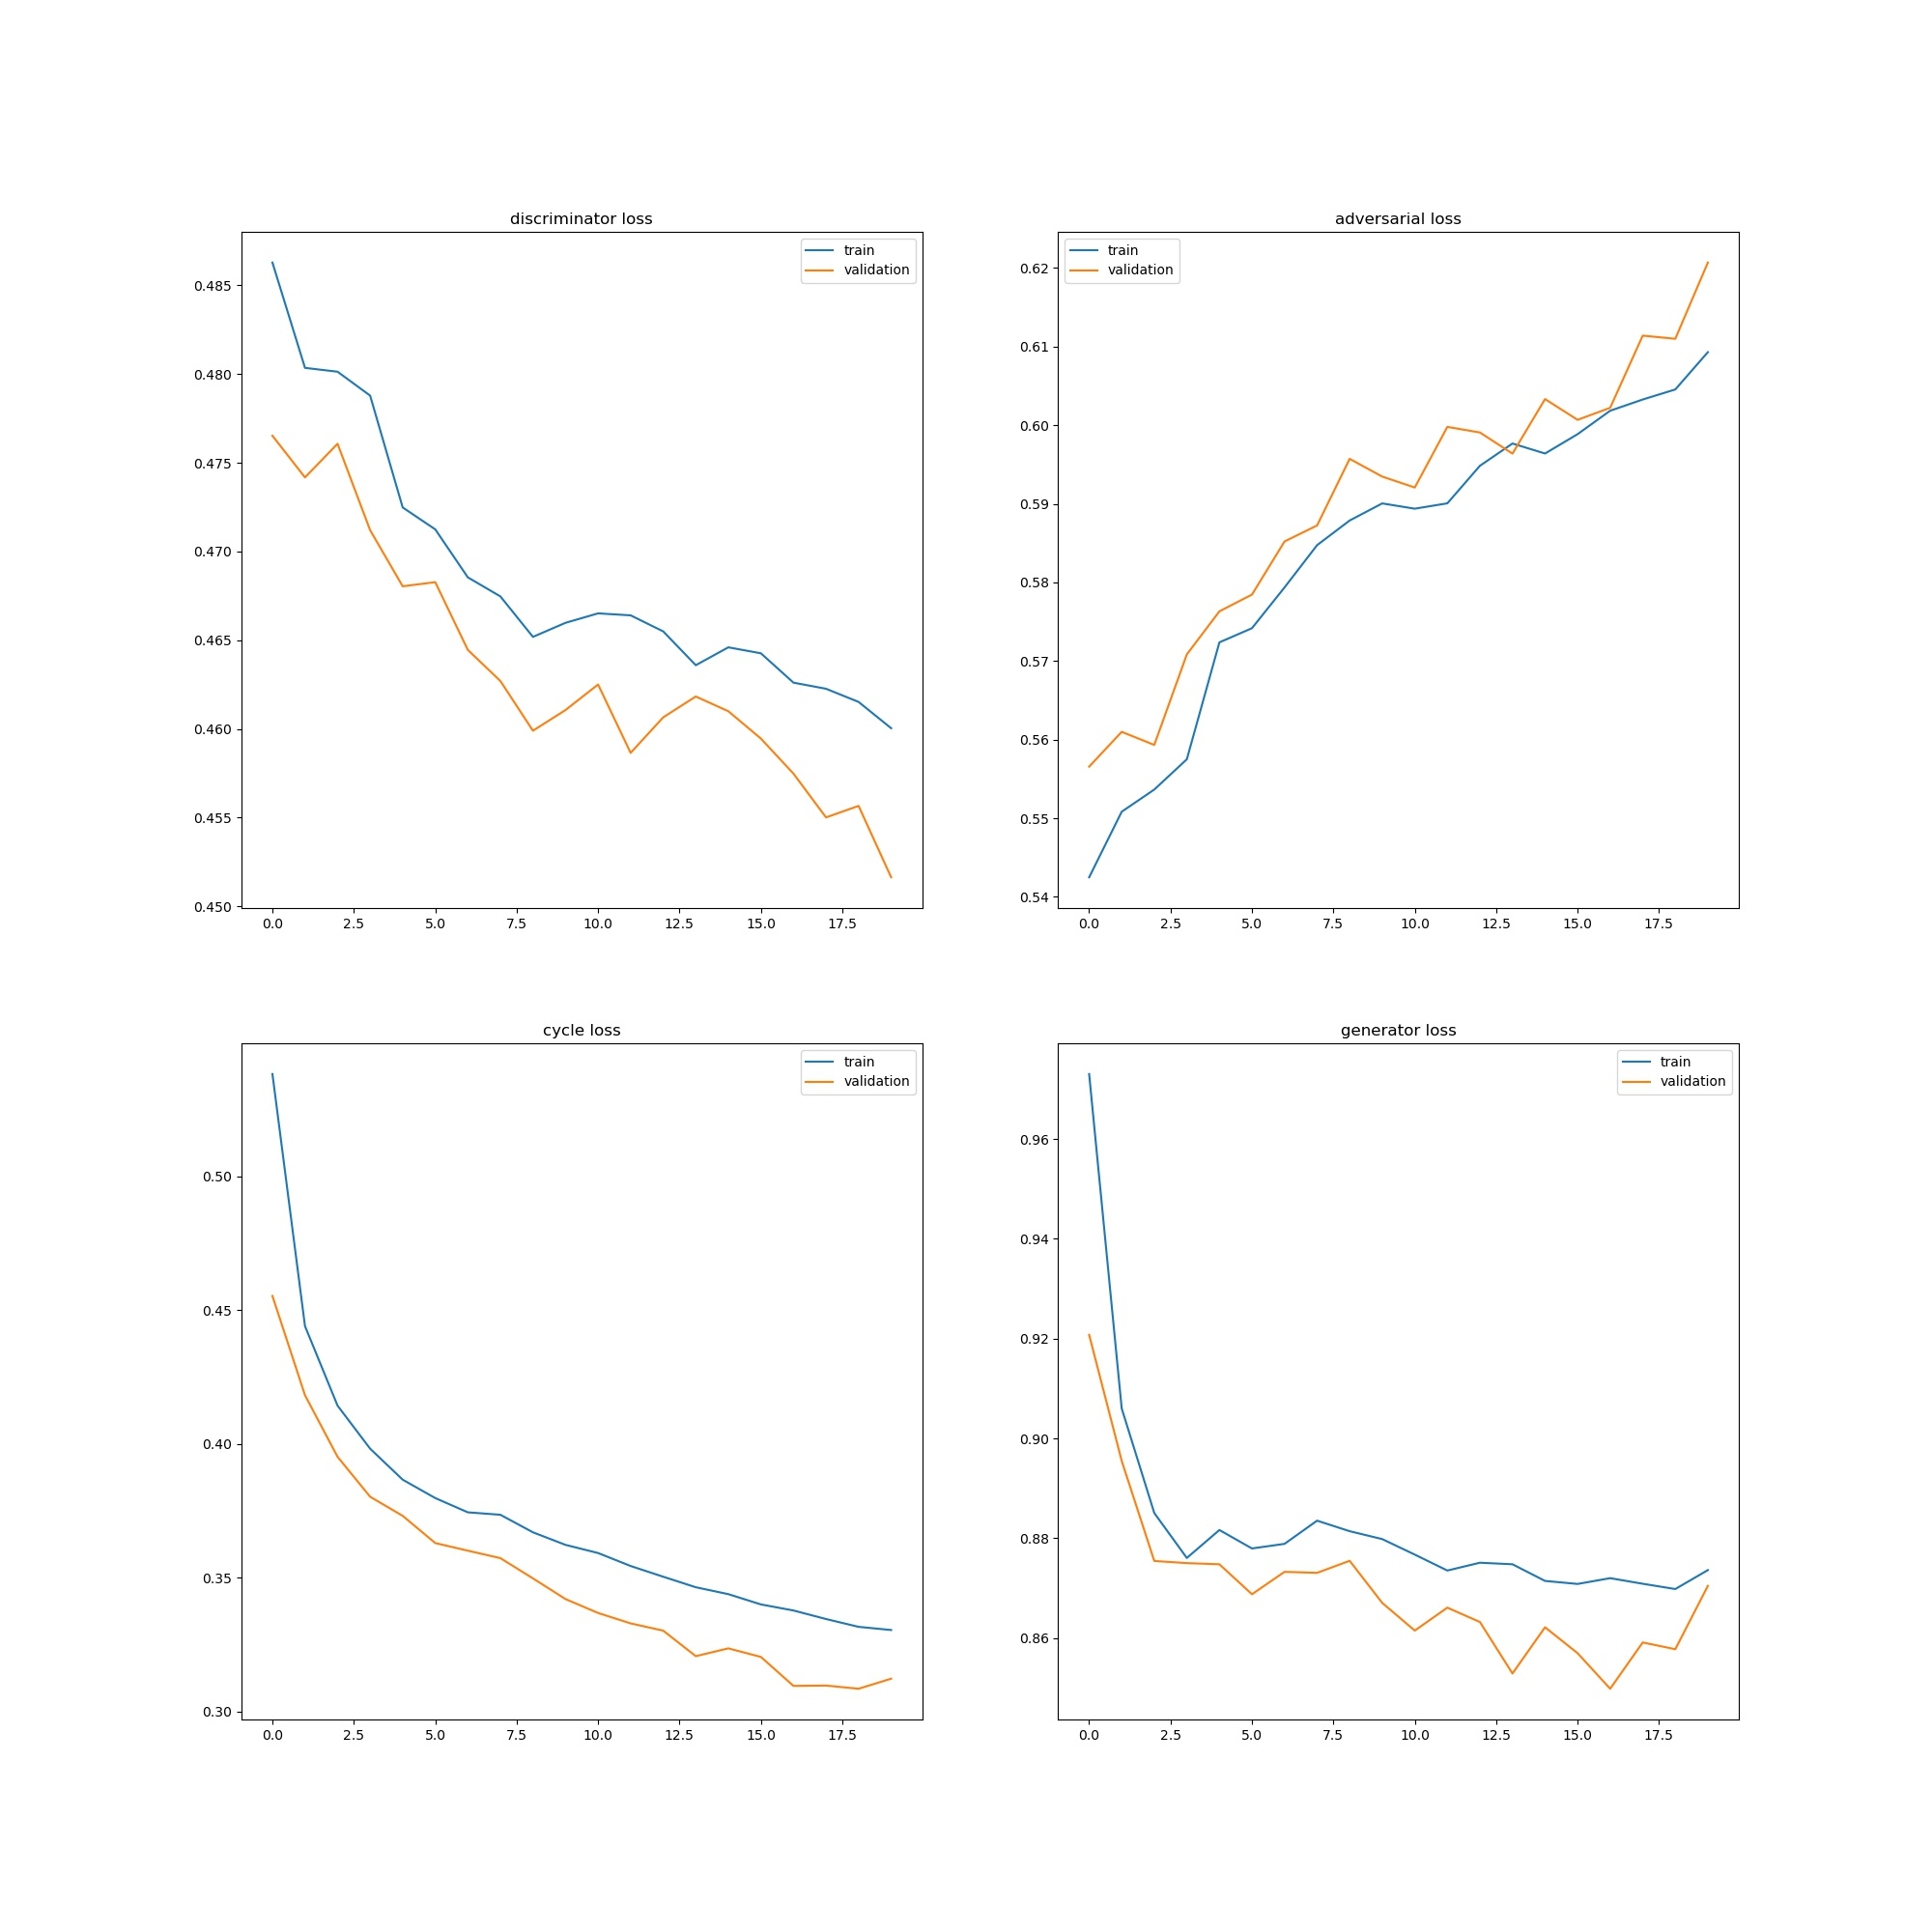
\includegraphics[width=10cm,height=10cm,keepaspectratio]{cycleGan/figures/logs/training_logs}

\caption{Training logs for CycleGan}
\end{figure}
\\
As witnessed in Figure 1, the adversarial loss is increasing but all
other losses are decreasing. The increase in adversarial loss can
have two possible causes:
\begin{enumerate}
\item The Generator may be too powerful compared to discriminator.
\item It may be due to the stochastic nature of training and further training
may remedy this problem.
\end{enumerate}
\item Here are a few images generated by the model:
\begin{figure}[h]
\subfloat[Generated images from A dataset(horse to zebra)]{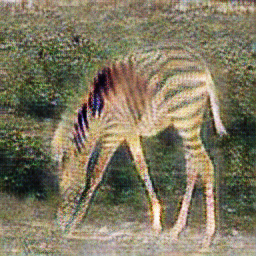
\includegraphics[width=3cm,height=3cm]{cycleGan/figures/train/A_epoch19_1200}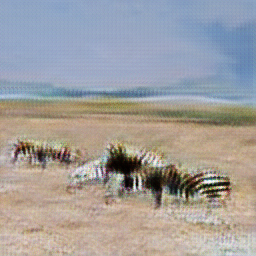
\includegraphics[width=3cm,height=3cm,keepaspectratio]{cycleGan/figures/train/A_epoch19_1000}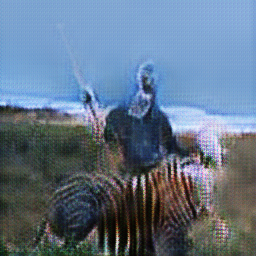
\includegraphics[width=3cm,height=3cm,keepaspectratio]{cycleGan/figures/train/A_epoch19_800}

}

\subfloat[Generated images from B dataset(zebra to horse)]{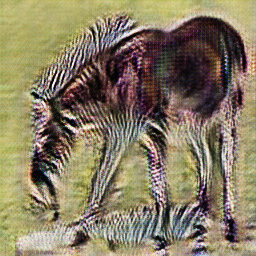
\includegraphics[width=3cm,height=3cm,keepaspectratio]{cycleGan/figures/train/B_epoch14_800}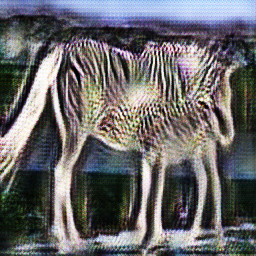
\includegraphics[width=3cm,height=3cm,keepaspectratio]{cycleGan/figures/train/B_epoch13_1000}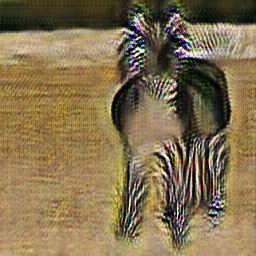
\includegraphics[width=3cm,height=3cm,keepaspectratio]{cycleGan/figures/train/B_epoch14_200}

}\caption{generated images by model}

\end{figure}
 As demonstrated in Figure 2, the model has better learned to turn
horses to zebras than vice versa. This can be fixed with further training.
\end{itemize}
\pagebreak{}

\section{Variational Auto Encoder}

\subsection{Stage 1}
\begin{itemize}
\item if the decoder is sufficiently powerful, then the training objective
can be solved with a dumb strategy: the encoder always produces $p(z)$
regardless of the data, and the decoder always produces $p(x)$ regardless
of $z$. The paper Neural Discrete Representation Learning (from van
den Oord and others from deepmind) calls this \textquotedbl posterior
collapse\textquotedbl .\\
Due to posterior collapse, VAEs cannot be controled since the decoder
ignores the latent space. This results in the VAE only producing a
limited set of outputs and not being able to generalize
\item In a GAN models, the generator may be able to learn one or a few pluseble
outputs which can decive the discriminator. However this is not desirable.
This phenomena can be remedied if the discriminator learns to distinguish
between real and fake inputs. However if the discriminator gets stuck
in a local minimum, it will not be able to solve the loophole that
the generator has discoverd and thus resulting in the GAN only generating
a few different output images. This phenomena is called ``mode collapse''.
The difference between ``model collapse'' and ``posterior collapse''
is that the former is cauesed due to under parameterized discriminator
but the latter is caused by over parameterized decoder.
\end{itemize}

\subsection{Stage 2}
\begin{itemize}
\item The VQ-VAE loss is 
\[
L=log(p(x|z_{q}(x))+\left\Vert sg\left[z_{e}(x)\right]-e\right\Vert _{2}^{2}+\beta\left\Vert z_{e}(x)-sg[e]\right\Vert _{2}^{2}
\]
The first term is the reconstruction loss which basically can be simplified
to an L2 loss between the input and the output assuming a Gaussian
data likelihood. This term is responsible for training the encoder
and the decoder(it is the auto encoder loss) and by removing this
term the encoder and the decoder cannot be trained. \\
The second term is pushing the code-book vectors to their corresponding
encoded vectors. SG is an abbreviation for stop gradient which means
detaching the argument from the computational graph. The embeddings
optimize this term hence by removing this part, training of the embeddings
is disrupted.\\
The last term pushes the encoded vectors to the code-book vectors(the
conjugate operation of the second term somehow). This term is a part
of training loss for the encoder and removing it will negatively effect
the training of the encoder part.
\item Auto-Regressive models work by feeding their regression output back
to model for the next prediction. First, the VQ-VAE is trained end
to end to learn how to reconstruct the images. Once the training is
done, the model has a fully trained encoder, decoder and code-book
vector set. After the training, to generate novel images, a special
token is passed to the predictor part and the predictor generates
a number. The generated number is then fed back to the predictor.
This operation is repeated until the latent space which is 32 by 32
in this case is filled with numbers. The model generates new images
based on the generated 32 by 32 matrix and the code-book vectors.
\item The prior distribution $p(z)$ is a uniform distribution and the posterior
distribution $p(z|x)$ is a single vector. This is due to discretization
of the posterior with the code-book vectors. If KL divergence between
the prior and the posterior is computed, the result would be
\[
1\times\log\left(\frac{1}{\frac{1}{k}}\right)=\log(k)
\]
$k$ is the length of the prior distribution.
\end{itemize}

\subsection{Stage 3}
\begin{itemize}
\item Figure 3 demonstrates training logs for 40 epochs:
\begin{figure}[h]
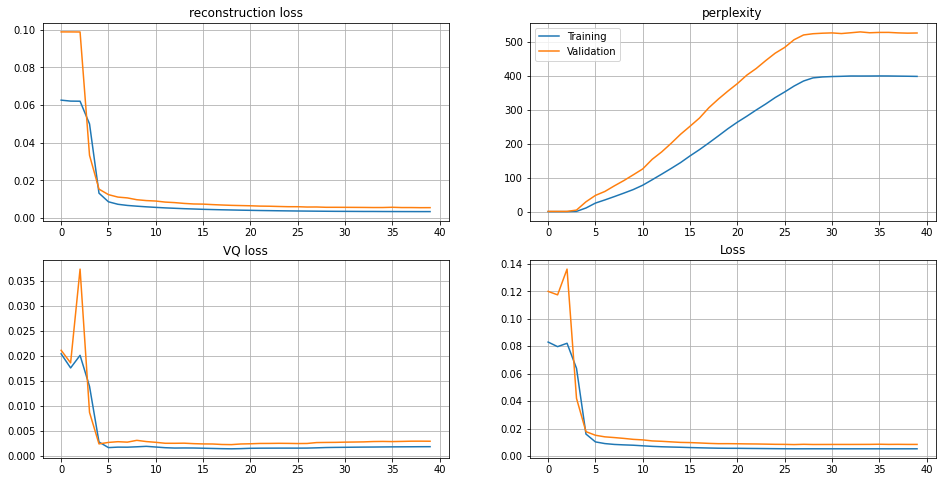
\includegraphics[width=10cm,height=10cm,keepaspectratio]{VQ_VAE/figures/training_logs}

\caption{Training logs for VQ-VAE}

\end{figure}
 It can be seen that both reconstruction loss and VQ loss are decreasing
and the perplexity, which is the utilization rate of the code-book
vectors, is increasing. after 40 epochs everything will converge.
Hence, 40 epochs was enough training. A UMAP abstraction of the embedding
vectors is illustrated in Figure 4:
\begin{figure}[H]
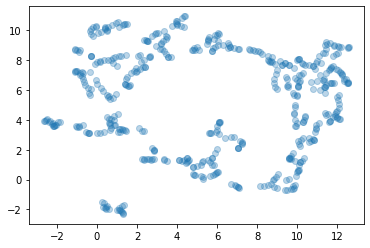
\includegraphics[width=10cm,height=10cm,keepaspectratio]{VQ_VAE/figures/cp_um}

\caption{UMAP representation of embedding vectors }

\end{figure}
 As clearly demonstrated in figure 4, there is a nice separation in
the embedding space which is a result of vector quantization.
\item Some reconstructed images are presented in Figure 5:
\begin{figure}[H]
\subfloat[Original]{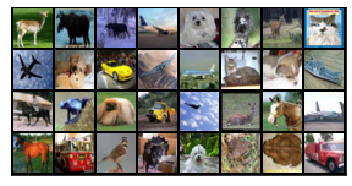
\includegraphics[width=5cm,height=5cm,keepaspectratio]{VQ_VAE/figures/val_original}

}\subfloat[Reconstructed ]{

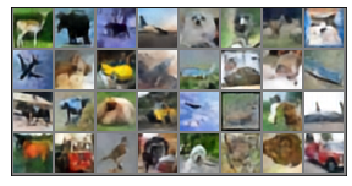
\includegraphics[width=5cm,height=5cm,keepaspectratio]{VQ_VAE/figures/val_recon}

}

\caption{Original vs reconstructed images from validation set}

\end{figure}
\end{itemize}

\end{document}
